% Preamble
\documentclass[11pt]{article}

% Packages
\usepackage{amsmath}
\usepackage{mathtools}
\usepackage{ragged2e}
\usepackage [utf8]{inputenc}
\usepackage{blindtext}
\usepackage{wrapfig}
\usepackage{xcolor}
\usepackage {polski}
\usepackage{multicol}
\usepackage[a4paper, total={5.7in, 8in}]{geometry}
\usepackage{graphicx}
\usepackage{amstex}
\usepackage{csvsimple}
\usepackage{changepage}
\usepackage{enumitem}
\usepackage[english]{babel}
\usepackage{biblatex}
\usepackage{caption}
\usepackage{indentfirst}
\usepackage{epstopdf-base}
\usepackage{textcomp}

% Document
\begin{document}
%    Nagłówek
\begin{flushleft}
        Maciej Pierzchała 282 934 \hfill Data wykonania ćwiczenia:\\
        Filip Kubecki 272 655 \hfill 26 października 2024r\\
        Grupa: Wtorek 10:35 \\
    \end{flushleft}

    \begin{center}
        \Large\textbf{Laboratorium 2}\\
        \textbf{Charakteryzacja czujników ciśnienia}
    \end{center}
    \hfill
%    Treść
    \section{Spis przyrządów}
    \par{
        Do wykonania ćwiczenia wykorzystano:
        \begin{itemize}
            \setlength\itemsep{0em}
            \item[-] Przetwornik ciśnienia Pt100
            \item[-] Przetwornik ciśnienia Pt101
            \item[-] Multimetr cyfrowy Sigilent SDM 3055
            \item[-] Cylinder pomiarowy
            \item[-] Kolumna do pomiaru ciśnienia wody wywieranej na przetworniki
        \end{itemize}
    }
    \section{Przebieg i cele doświadczenia}
    \par Celem ćwiczenia jest zapoznianie się z budową oraz zasadą działania przetworników ciśnienia z czujnikiem piezorezystancyjnym
    oraz wyznaczenie gęstości wody na podstawie pomiaru ciśnienia hydrostatycznego.\\
    \indent Pominięto pomiar dla objętości 1600 [ml] gdyż ciecz nie mieściła się w kolumnie pomiarowej. Poniżej przedstawiono schemat układu pomiarowego jaki zastosowano w ćwiczeniu:\\
    \noindent\makebox[\textwidth]{
        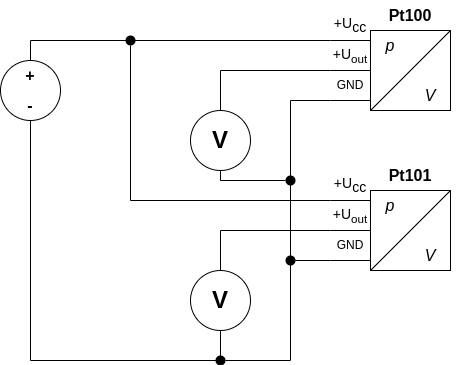
\includegraphics[scale = 0.55]{/home/bork/IdeaProjects/LatexProjects/src/PodstawyTechnikiSensorowej/Lab2/Img/schematic.png}}
    \section{Obliczenia i analiza wyników}
   \par\noindnet Poniżej umieszczone zostają parametry sali w której przeprowadzano doświdczenie:
    \begin{gather*}
        p=1009.9 [hPa]\\
        T=25.24 [^\circ C]\\
        RH=51.8 [\%]
    \end{gather*}
    \noindent Ciśnienie w oparciu o sygnał wyjściowy przetwornika ciśnienia wyliczamy z poniższego wzoru:
    \begin{gather}
        p=\frac{p_{max}-p_{min}}{U_{max}-U_{min}}\cdot U_{out}+p_{min}
    \end{gather}
    \noindent Gdzie:
        {\footnotesize
    \begin{itemize}
        \setlength\itemsep{0em}
        \item[] \textbf{$p$} - ciśnienie mierzone,
        \item[] \textbf{$p_{max}, p_{min}$} - wartość maksymalna i minimalna zakresu pomiaru ciśnienia dla przetwornika,
        \item[] \textbf{$U_{max}, U_{min}$} - wartość maksymalna i minimalna zakresu napięcia wyjściowego dla przetwornika,
        \item[] \textbf{$U_{out}$} - napięcie wyjściowe przetwornika,
    \end{itemize}}
    \noindent Przykładowo dla czujnika Pt100 dla ciśnienia atmosferycznego:
    \begin{gather}
        p=\frac{1.15 [bar] - 0.95 [bar]}{10[V]}\cdot 2.97[V]+0.95[bar]=1.0094 [bar]=1009.4 [hPa]
    \end{gather}
    \noindent Dla czujnika Pt101 dla ciśnienia atmosferycznego:
    \begin{gather}
        p=\frac{0.1 [bar]}{10[V]}\cdot 44.9[mV]=0.000449 [bar]=0.449 [hPa]
    \end{gather}
    \noindent Wysokość słupa wody wyliczono przekształcając wzór na objętość walca:
    \begin{gather}
        V=P_p\cdot h=\pi\cdot r^2\cdot h
    \end{gather}
    \noindent Gdzie:
        {\footnotesize
    \begin{itemize}
        \setlength\itemsep{0em}
        \item[] \textbf{$V$} - objętość walca (w naszym przypadku objętość dolewanej wody),
        \item[] \textbf{$h$} - wysokość walca (w naszym przypadku słupa cieczy),
        \item[] \textbf{$P_p$} - pole podstawy,
        \item[] \textbf{$r$} - promień walca,
    \end{itemize}}
    \noindent Przekształcając:
    \begin{gather}
        V=\pi\cdot r^2\cdot h\quad \bigg/\ \pi\cdot r^2 \\
        h=\frac{V}{\pi\cdot r^2}
    \end{gather}
    \noindent Dla naszego walca wysokość słupa cieczy przy dolaniu $100 [ml]$ wody wynosi:
    \begin{gather}
        h=\frac{100 [ml]}{\pi\cdot (\frac{45[mm]}{2})^2}=\\
        =\frac{100 [cm^3]}{15.904312 [cm^2]}=6.2876\dots [cm]
    \end{gather}
%    Tutaj wykresy
    \newpage
    Na podstawie danych uzyskanych przy pomocy powyższych wzorów wyznaczono wykresy zależności $p=f(h)$ dla obu
    przetworników:\\
    \noindent\makebox[\textwidth]{
        \includegraphics[scale = 0.42]{/home/bork/IdeaProjects/LatexProjects/src/PodstawyTechnikiSensorowej/Lab2/Img/Pt100.png}}
    \noindent\makebox[\textwidth]{
        \includegraphics[scale = 0.42]{/home/bork/IdeaProjects/LatexProjects/src/PodstawyTechnikiSensorowej/Lab2/Img/Pt101.png}}
%    Gęstość
    \noindent Gęstość wody wyznaczamy z równiania:
    \begin{gather}
        a=\rho g
    \end{gather}
    \noindent Gdzie:
    {\footnotesize
        \begin{itemize}
            \setlength\itemsep{0em}
            \item[] \textbf{$a$} - współczynnik kierunkowy zależności p=f(h),
            \item[] \textbf{$\rho$} - gęstość wody,
            \item[] \textbf{$g$} - przyśpieszenie ziemskie (przyjmujemy 9.81 [$\frac{m}{s^2}$]),
        \end{itemize}}
    \noindent Gęstość wody będzie przedstawiona wzorem:
    \begin{gather}
        \rho=\frac{a}{g}
    \end{gather}
    \noindent Dla czujnika Pt100:
    \begin{gather}
        \rho=\frac{97.62011 [\frac{Pa}{cm}]}{9.81[\frac{m}{s^2}]}=9.951082 [\frac{kg}{cm\cdot m^2}]=\\
        =995.1082 [\frac{kg}{m^3}]
    \end{gather}
    \noindent Dla czujnika Pt101:
    \begin{gather}
        \rho=999.527 [\frac{kg}{m^3}]
    \end{gather}

    \section{Wnioski}
    \par Dla wody w temperaturze $25 [^\circ C]$ gęstość wynosi $997 [\frac{kg}{m^3}]$. Możemy więc stwierdzić że wartości
    wyznaczone w doświdczeniu są poprawne. Lekkie odbieganie wartości obliczonych od wartości tablicowej może wynikać z niedokładności
    odczytu objętości wody wlewanej do cylindra oraz z niepewności wynikających z parametrów doświadczenia.

    %Bibliografia
    \vfill
    \footnotesize
    \begin{thebibliography}{3}
        \bibitem{texbook1}
        https://en.wikipedia.org/wiki/Pressure
        \bibitem{texbook2}
        https://en.wikipedia.org/wiki/MEMS
        \bibitem{texbook3}
        https://pubchem.ncbi.nlm.nih.gov/substance/329798917
    \end{thebibliography}

%   Data
    \newpage
% TODO: Add reference data
    \begin{center}
        \Large\csvreader[tabular = |c|c|c|c|c|c|,
            table head = \hline  \textbf{V[ml]} & \textbf{h[cm]} & \textbf{\boldmath$p_{pt100}$[bar]} & \textbf{\boldmath$p_{pt100}$[Pa]} & \textbf{\boldmath$p_{pt101}$[bar]} & \textbf{\boldmath$p_{pt101}$[Pa]} \\\hline,
%            table foot = \hline,
            late after line = \\\hline
        ]{Data/oData.csv}{}{
            \csvcoli & \csvcolii & \csvcoliii & \csvcoliv  & \csvcolv & \csvcolvi
        }
    \end{center}
\end{document}